\documentclass[a4paper, 12pt]{article}

\def\languages{french, english}

%%%%%%%%%%%%%%%%%%% Libraries

%%%%%%%%%% Packages

\usepackage[
backend=biber,
style=numeric-comp,
sorting=none,
maxbibnames=99
]{biblatex}

%%%%%%%%%% Packages

%%%%% Coding tools

\usepackage{comment}
\usepackage{xstring}

%%%%% Encoding

\usepackage[utf8]{inputenc}
\usepackage[T1]{fontenc}
\usepackage{eurosym}

%%%%% Languages

\ifx\languages\undefined
	\usepackage[english]{babel}
\else
	\usepackage[\languages]{babel}
\fi

\def\languagefile{./include/languages/\languagename.tex}
\InputIfFileExists{\languagefile}{}

%%%%% Style

\usepackage{geometry}
\usepackage{fancyhdr}
\usepackage[bottom]{footmisc}

\edef\restoreparindent{\parindent=\the\parindent\relax}
\usepackage[parfill]{parskip}

\usepackage{enumitem}
\usepackage{csquotes}
\usepackage{color}

%%%%% Others

\usepackage[framemethod=TikZ]{mdframed}
\usepackage[pdfusetitle]{hyperref}

%%%%%%%%%% Features

%%%%% Settings

\geometry{paper=a4paper,top=3.5cm,bottom=2.5cm,right=2.5cm,left=2.5cm}

\pagestyle{fancy}
\fancyhead[L]{}
\fancyhead[R]{\leftmark}
\fancyfoot[C]{\thepage}
\renewcommand{\headrulewidth}{0pt}

%\restoreparindent

%%%%% Commands

\newcommand{\romantableofcontents}{
	\newpage
	\pagenumbering{roman}
	\tableofcontents
	\newpage
	\pagenumbering{arabic}
}

%%%%%%%%%% Packages

\usepackage{float}
\usepackage[skip=1em]{caption}

\usepackage{array}
\usepackage{multirow}
\usepackage{multicol}

%%%%%%%%%% Features

%%%%% Settings

\renewcommand{\arraystretch}{1.2}

%%%%% Commands

\newcommand\noskipcaption[1]{\caption{#1}\vspace{-1em}}

%%%%%%%%%% Packages

\usepackage{inconsolata}
\usepackage{listings}

%%%%%%%%%% Features

%%%%% Commands

\newcommand{\Nstyle}[1]{
    \lstdefinestyle{N#1}{
        style=#1,
        %%%%%
        numbers=left
    }
}

\newcommand{\tbFstyle}[1]{
    \lstdefinestyle{tbF#1}{
        style=#1,
        %%%%%
        frame=tb
    }
}

\newcommand{\Fstyle}[1]{
    \lstdefinestyle{F#1}{
        style=#1,
        %%%%%
        frame=single,
        framesep=0em,
        rulesep=0em,
        xleftmargin=0.75em,
        xrightmargin=0.75em,
        framexleftmargin=0.75em,
        framexrightmargin=0.75em,
        framextopmargin=0.5em,
        framexbottommargin=0.5em,
        %%%%%
        numbersep=1.25em
    }
}

\newcommand{\NtbFstyle}[1]{
    \tbFstyle{#1}
    \Nstyle{tbF#1}
}

\newcommand{\NFstyle}[1]{
    \Fstyle{#1}
    \lstdefinestyle{NF#1}{
        style=f#1,
        %%%%%
        xleftmargin=2.75em,
        framexleftmargin=2.75em,
        %%%%%
        numbers=left,
        numbersep=1em
    }
}

%%%%% Styles

\lstdefinestyle{default}{
    breaklines=true,
    breakatwhitespace=true,
    columns=fixed,
	extendedchars=true,
    upquote=true,
	tabsize=4,
    %%%%%
    framerule=0.66pt,
    captionpos=b,
	%%%%%
    basicstyle=\footnotesize\ttfamily,
    numberstyle=\footnotesize\ttfamily,
    showstringspaces=false
}
\Nstyle{default}
\NFstyle{default}
\NtbFstyle{default}

\lstdefinestyle{monokai}{
    style=Fdefault,
    %%%%%
    backgroundcolor=\color[HTML]{272822},
    framerule=0em,
    %%%%%
    basicstyle=\footnotesize\ttfamily\color[HTML]{f8f8f2},
    numberstyle=\footnotesize\ttfamily\color[HTML]{272822},
    commentstyle=\color[HTML]{75715e},
    keywordstyle=[1]{\color[HTML]{f92672}},
    keywordstyle=[2]{\color[HTML]{A6E22E}},
    keywordstyle=[3]{\color[HTML]{ae81ff}},
    stringstyle=\color[HTML]{e6db74},
    %%%%%
    % otherkeywords={!,.,+,-,*,/,=,<,>,^,|,\&,OR,AND}
}

\lstdefinestyle{Nmonokai}{
    style=monokai,
    %%%%%
    xleftmargin=2.75em,
    framexleftmargin=2.75em,
    %%%%%
    numbers=left,
    numberstyle=\footnotesize\ttfamily\color[HTML]{f8f8f2},
    numbersep=1em
}

\lstdefinestyle{c}{
    language=C,
    style=default,
    %%%%%
    commentstyle=\color[HTML]{228B22},
    keywordstyle=\color[HTML]{0000FF},
    stringstyle=\color[HTML]{A020F0},
    emphstyle=\color[HTML]{0000FF},
    %%%%%
    emph={}
}

\lstdefinestyle{cpp}{
    language=C++,
    style=default,
    %%%%%
    commentstyle=\color[HTML]{228B22},
    keywordstyle=\color[HTML]{0000FF},
    stringstyle=\color[HTML]{A020F0},
    emphstyle=\color[HTML]{0000FF},
    %%%%%
    emph={std}
}

\lstdefinestyle{matlab}{
    language=matlab,
    style=default,
    %%%%%
    basicstyle=\footnotesize\fontfamily{pcr}\selectfont,
    numberstyle=\footnotesize\fontfamily{pcr}\selectfont,
    commentstyle=\color[HTML]{228B22},
    keywordstyle=\color[HTML]{0000FF},
    stringstyle=\color[HTML]{A020F0},
    emphstyle=\color[HTML]{0000FF},
    %%%%%
    emph={clearvars}
}

\lstdefinestyle{python}{
    language=python,
    style=default,
    %%%%%
    commentstyle=\color[RGB]{221,0,0},
    keywordstyle=[1]{\color[RGB]{255,119,0}},
    keywordstyle=[2]{\color[RGB]{144,0,144}},
    stringstyle=\color[RGB]{0,170,0},
    emphstyle=\color[RGB]{255,119,0},
    %%%%%
    emph={}
}

\lstdefinestyle{java}{
    language=java,
    style=default,
    %%%%%
    commentstyle=\color[HTML]{228B22},
    keywordstyle=\color[HTML]{0000FF},
    stringstyle=\color[HTML]{A020F0},
    emphstyle=\color[HTML]{0000FF},
    %%%%%
    emph={}
}

%%%%%%%%%% Packages

\usepackage{amsmath}
\usepackage{amssymb}
\usepackage{bm}
\usepackage{esint}
\usepackage[makeroom]{cancel}

%%%%%%%%%% Features

%%%%% Macros

\newcommand{\rbk}[1]{\left(#1\right)}
\newcommand{\cbk}[1]{\left\{#1\right\}}
\newcommand{\sbk}[1]{\left[#1\right]}
\newcommand{\abs}[1]{\left|#1\right|}
\newcommand{\norm}[1]{\left\|#1\right\|}

\newcommand{\fact}[1]{#1!}
\newcommand{\e}[1]{\mathbf{e}_{#1}}
\newcommand{\deriv}{\mathrm{d}}
\DeclareMathOperator{\tr}{tr}

\def\Rl{\mathbb{R}}
\def\Cx{\mathbb{C}}
\def\Na{\mathbb{N}}
\def\Zi{\mathbb{Z}}

%%%%%%%%%% Packages

\usepackage{amsthm}
\usepackage{thmtools}

%%%%%%%%%% Features

%%%%% Settings

\makeatletter
\define@key{thmdef}{mdthm}[{}]{
	\thmt@trytwice{\def\thmt@theoremdefiner{\mdtheorem[#1]}}{}}
\makeatother

\begingroup
\makeatletter
\@for\theoremstyle:=plain,definition,remark\do{
	\expandafter\g@addto@macro\csname th@\theoremstyle\endcsname{
		\addtolength\thm@preskip\parskip
	}
}
\endgroup

\renewcommand{\qedsymbol}{$\blacksquare$}

% language

\ifx\lgthm\undefined
	\def\lgthm{Theorem}
	\def\lgprf{Proof}
	\def\lglem{Lemma}
	\def\lgprop{Proposition}
	\def\lgdefn{Definition}
	\def\lghyp{Hypothesis}
	\def\lgmeth{Method}
	\def\lgquest{Question}
	\def\lgansw{Answer}
	\def\lgexpl{Example}
	\def\lgrmk{Remark}
	\def\lgnote{Note}
	\def\lgtip{Tip}
\fi

%%%%% Commands

\newcommand\qedadd{\pushQED{\qed}\popQED}

%%%%% Environments

\theoremstyle{plain}
\newtheorem{thm}{\lgthm}
\newtheorem{lem}[thm]{\lglem}
\newtheorem{prop}[thm]{\lgprop}

\theoremstyle{definition}
\newtheorem{defn}{\lgdefn}
\newtheorem{hyp}{\lghyp}
\newtheorem{meth}{\lgmeth}
\newtheorem{quest}{\lgquest}

\theoremstyle{remark}
\newtheorem{answ}{\lgansw}[quest]
\newtheorem{expl}{\lgexpl}
\newtheorem*{rmk}{\lgrmk}
\newtheorem*{note}{\lgnote}
\newtheorem*{tip}{\lgtip}

% framed

\mdfdefinestyle{thicc}{
	nobreak=true,
	skipabove=\topskip,
	skipbelow=\topskip,
	innerleftmargin=0.5em,
	innerrightmargin=0.5em,
	innerbottommargin=0.5em,
	innertopmargin=0.5em,
	linewidth=0.25em,
	roundcorner=0.15em,
	linecolor=black!10,
	frametitlebackgroundcolor=black!10,
	theoremseparator={.}
}

\declaretheorem[mdthm={style=thicc, linecolor=red!20, frametitlebackgroundcolor=red!20}, sibling=thm, name=\lgthm]{framedthm}
\declaretheorem[mdthm={style=thicc, linecolor=red!20, frametitlebackgroundcolor=red!20}, sibling=thm, name=\lglem]{framedlem}
\declaretheorem[mdthm={style=thicc, linecolor=blue!20, frametitlebackgroundcolor=blue!20}, sibling=thm, name=\lgprop]{framedprop}
\declaretheorem[mdthm={style=thicc, nobreak=false}, parent=thm, name=\lgprf]{framedprf}

\declaretheorem[mdthm={style=thicc, linecolor=black!20!green!20, frametitlebackgroundcolor=black!20!green!20}, sibling=defn, name=\lgdefn]{frameddefn}
\declaretheorem[mdthm={style=thicc, linecolor=blue!20, frametitlebackgroundcolor=blue!20}, sibling=hyp, name=\lghyp]{framedhyp}
\declaretheorem[mdthm={style=thicc}, name=\lgmeth]{framedmeth}
\declaretheorem[mdthm={style=thicc, linecolor=orange!20, frametitlebackgroundcolor=orange!20}, sibling=quest, name=\lgquest]{framedquest}

\declaretheorem[mdthm={style=thicc, nobreak=false}, sibling=answ, name=\lgansw]{framedansw}
\declaretheorem[mdthm={style=thicc, nobreak=false}, sibling=expl, name=\lgexpl]{framedexpl}

%%%%%%%%%% Packages

\usepackage{siunitx}

%%%%%%%%%% Features

%%%%% Settings

\ifx\decimalsign\undefined
\else
    \sisetup{output-decimal-marker = \decimalsign}
\fi


%%%%% Settings

% lists
\frenchbsetup{StandardLists=true}

% units
\def\decimalsign{,}

% captions
\addto\captionsfrench{\def\figurename{Figure}}
\addto\captionsfrench{\def\tablename{Table}}
\addto\captionsfrench{\def\proofname{Preuve}}

% theorems

\def\lgthm{Théorème}
\def\lgprf{Preuve}
\def\lglem{Lemme}
\def\lgprop{Proposition}
\def\lgdefn{Définition}
\def\lghyp{Hypothèse}
\def\lgmeth{Méthode}
\def\lgquest{Question}
\def\lgansw{Réponse}
\def\lgexpl{Exemple}
\def\lgrmk{Remarque}
\def\lgnote{Note}
\def\lgtip{Conseil}

%%%%% Macros

\def\tq{\text{t.q.}}
\def\cad{c.-à-d.}
\def\Cad{C.-à-d.}


%%%%%%%%%%%%%%%%%%% Titlepage

\def\logopath{resources/pdf/logo-uliege.pdf}
\def\toptitle{University of Liège}
\title{Homework 2}
\def\subtitle{Applied digital signal processing}
%\def\authorhead{Author}
\author{
    Quentin \textsc{Graillet}\\
    Maxime \textsc{Meurisse}\\
    Adrien \textsc{Schoffeniels}\\
}
%\def\rightauthorhead{}
%\def\rightauthor{}
\def\context{3\ieme{} year of Bachelor Civil Engineer}
\date{Academic year 2018-2019}

%%%%%%%%%%%%%%%%%%%

\fancyhead[R]{}
\NFstyle{matlab}

%%%%%%%%%%%%%%%%%%%

\begin{document}
	%%%%%%%%%% Packages

%%%%% Coding tools

\usepackage{comment}
\usepackage{xstring}

%%%%% Encoding

\usepackage[utf8]{inputenc}
\usepackage[T1]{fontenc}
\usepackage{eurosym}

%%%%% Languages

\ifx\languages\undefined
	\usepackage[english]{babel}
\else
	\usepackage[\languages]{babel}
\fi

\def\languagefile{./include/languages/\languagename.tex}
\InputIfFileExists{\languagefile}{}

%%%%% Style

\usepackage{geometry}
\usepackage{fancyhdr}
\usepackage[bottom]{footmisc}

\edef\restoreparindent{\parindent=\the\parindent\relax}
\usepackage[parfill]{parskip}

\usepackage{enumitem}
\usepackage{csquotes}
\usepackage{color}

%%%%% Others

\usepackage[framemethod=TikZ]{mdframed}
\usepackage[pdfusetitle]{hyperref}

%%%%%%%%%% Features

%%%%% Settings

\geometry{paper=a4paper,top=3.5cm,bottom=2.5cm,right=2.5cm,left=2.5cm}

\pagestyle{fancy}
\fancyhead[L]{}
\fancyhead[R]{\leftmark}
\fancyfoot[C]{\thepage}
\renewcommand{\headrulewidth}{0pt}

%\restoreparindent

%%%%% Commands

\newcommand{\romantableofcontents}{
	\newpage
	\pagenumbering{roman}
	\tableofcontents
	\newpage
	\pagenumbering{arabic}
}

	\section{Noise elimination}
	An electrocardiogram signal (\texttt{hw2\_electrocardiogram.mat}) is given with a sampling frequency of \SI{250}{\hertz}. This signal is noisy. The goal is to find the original signal, without the noise.\par
	The Matlab code used is appended to this document.
	\subsubsection*{Question (a)}
	First, we plot the entire signal (figure \ref{fig:plot_a}).
	\begin{figure}[H]
	    \centering
	    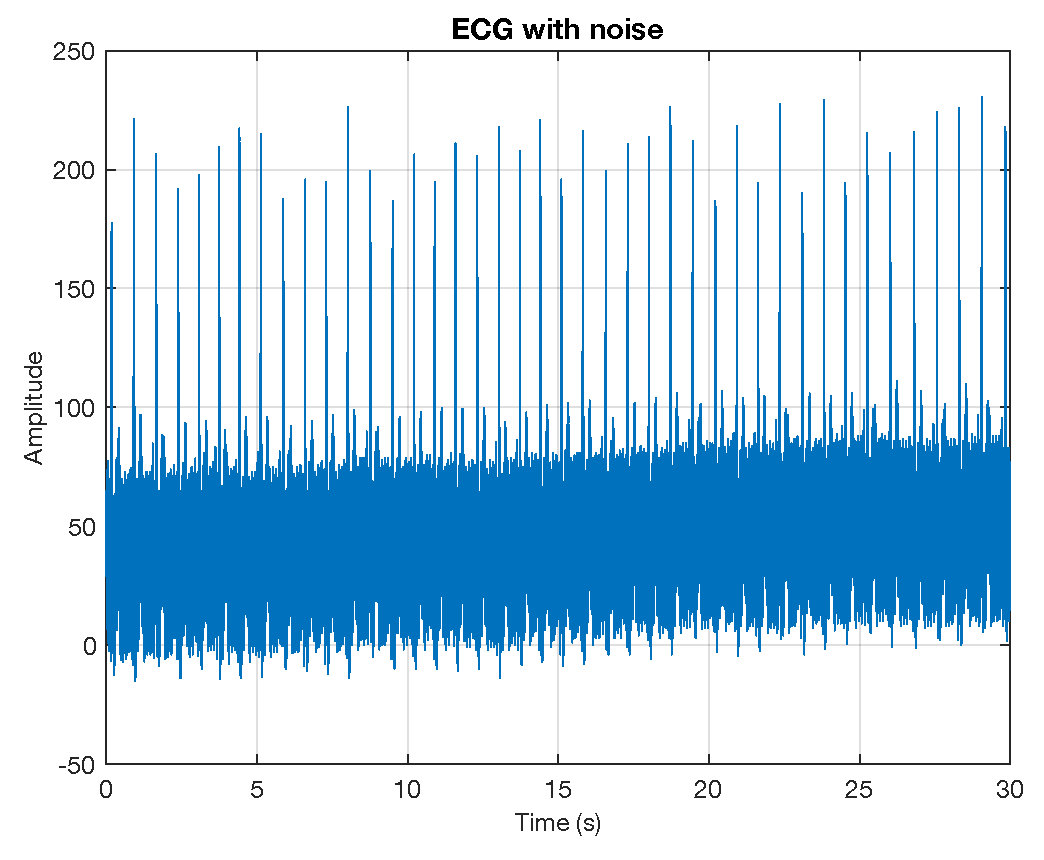
\includegraphics[width=0.9\textwidth]{resources/pdf/plot_a.pdf}
	    \caption{Whole signal as a function of time (in seconds)}
	    \label{fig:plot_a}
	\end{figure}
	\subsubsection*{Question (b)}
	Since the entire signal is not very visible, we only plot the signal between times 2 and 5 seconds (figure \ref{fig:plot_b}).
	\begin{figure}[H]
	    \centering
	    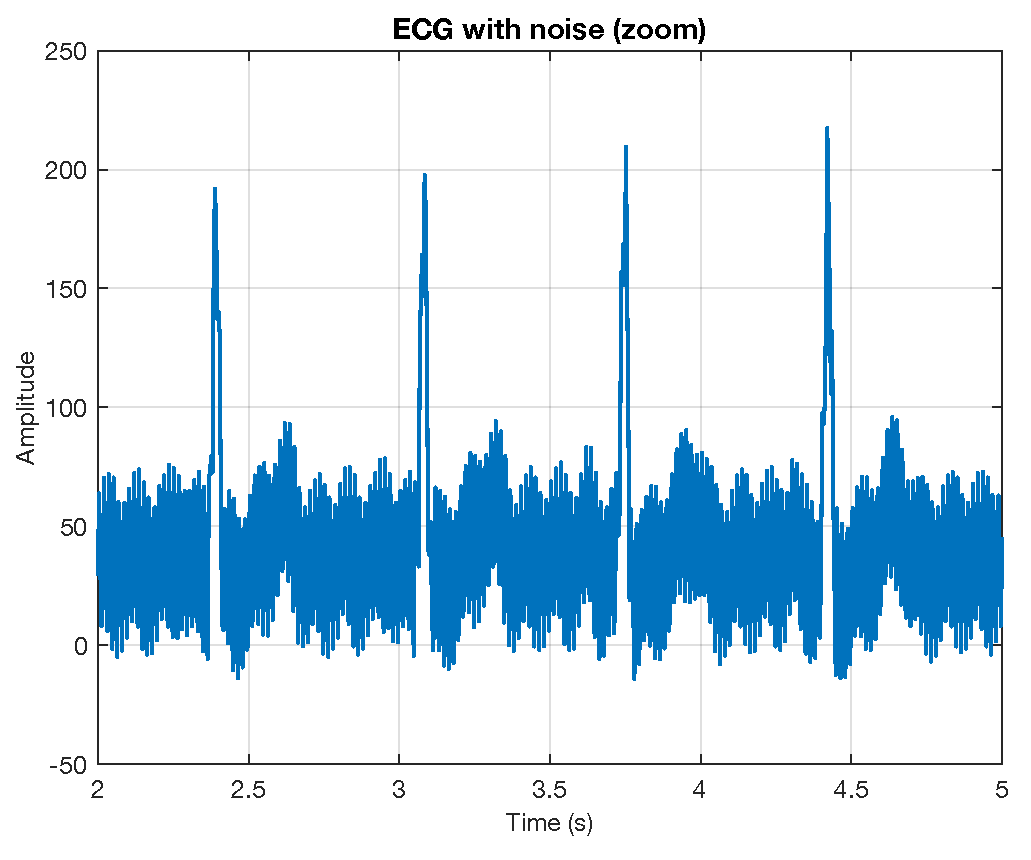
\includegraphics[width=0.9\textwidth]{resources/pdf/plot_b.pdf}
	    \caption{Signal between times 2 and 5 seconds}
	    \label{fig:plot_b}
	\end{figure}
	\subsubsection*{Question (c)}
	It is clearly observed that the signal is noisy. In order to identify the noisy frequencies, we plot the single-sided magnitude spectrum (thanks to the function \texttt{fft} of Matlab) of the signal (figure \ref{fig:plot_c}).
	\begin{figure}[H]
	    \centering
	    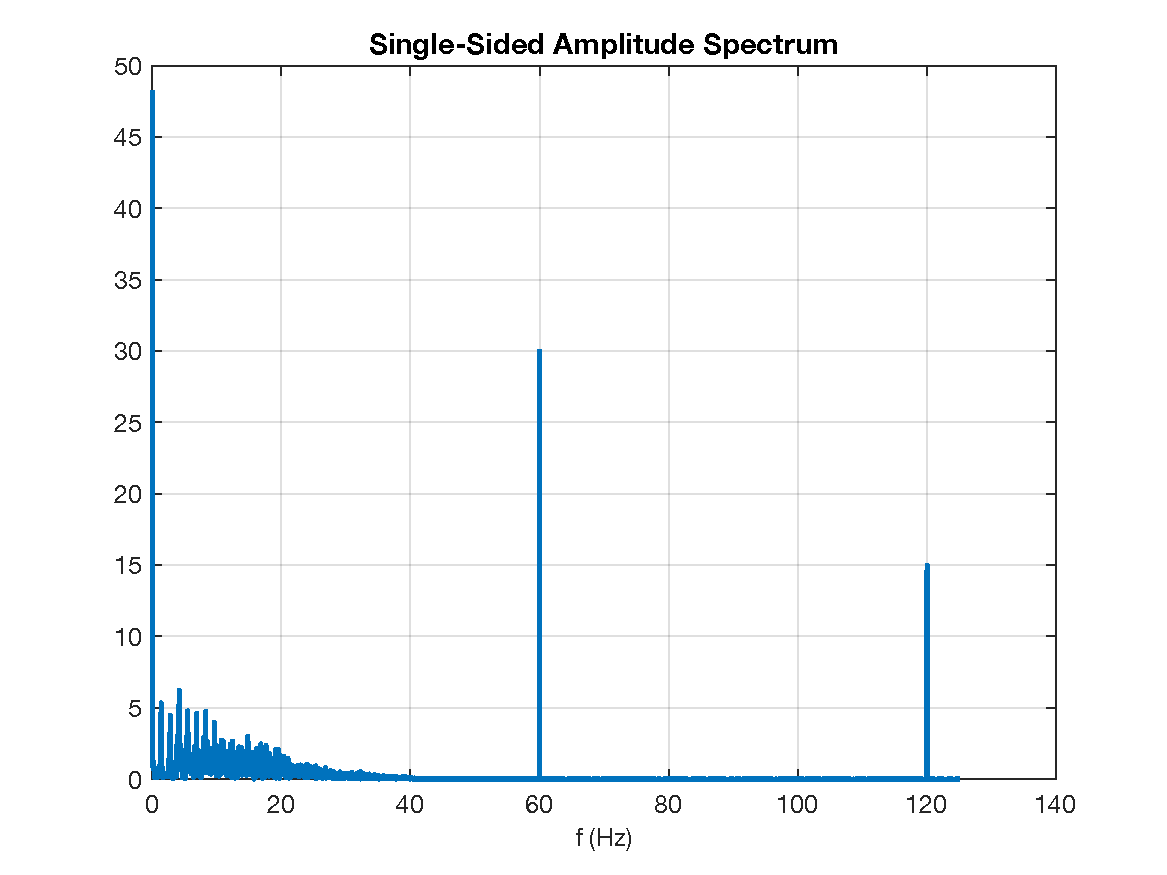
\includegraphics[width=0.9\textwidth]{resources/pdf/plot_c.pdf}
	    \caption{Single-sided magnitude spectrum of the signal}
	    \label{fig:plot_c}
	\end{figure}
	\subsubsection*{Question (d)}
	The two noisy frequencies are clearly identified by the two peaks: \SI{60}{\hertz} and \SI{120}{\hertz}.
	\subsubsection*{Question (e)}
	Both signals (noisy and non-noisy) are shown in figure \ref{fig:plot_e}.
	\begin{figure}[H]
	    \centering
	    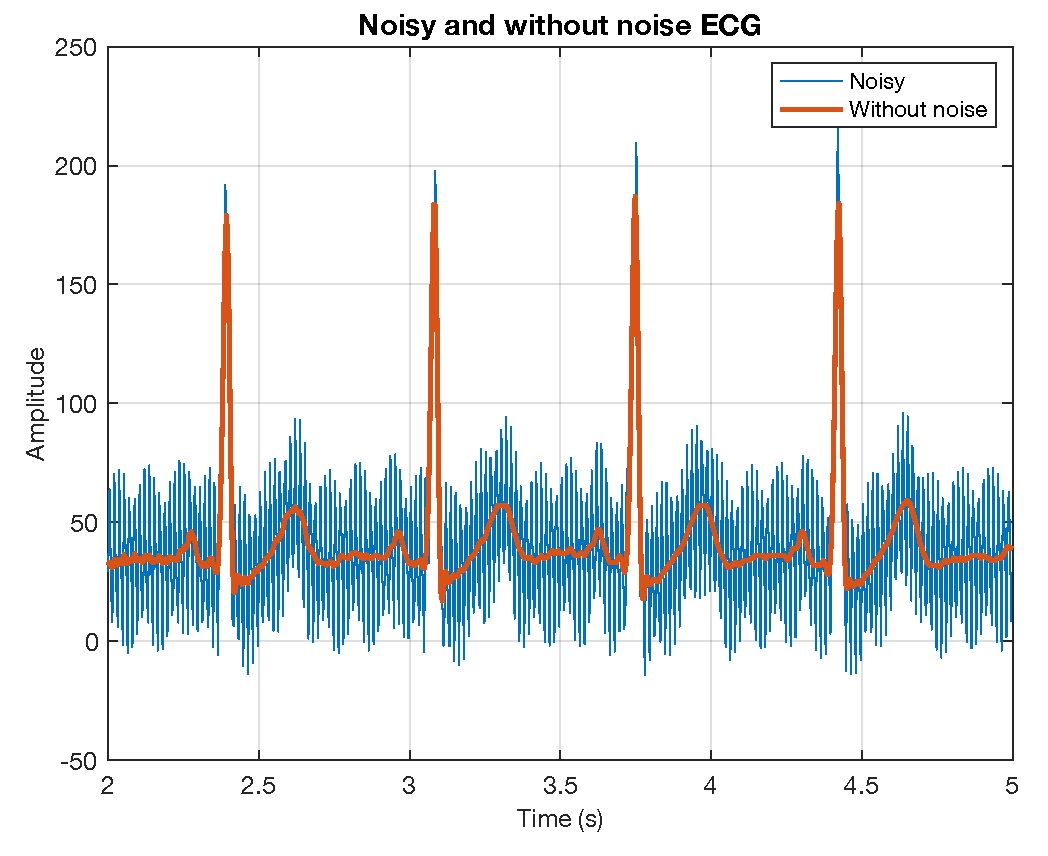
\includegraphics[width=0.9\textwidth]{resources/pdf/plot_e.pdf}
	    \caption{Noisy and original signal (from the second 2 to second 5)}
	    \label{fig:plot_e}
	\end{figure}
	\subsubsection*{Question (f)}
	We can create notch filters to filter the noisy frequencies. Indeed, a notch filter makes it possible to filter particular frequencies.\par
	In our case, we create two filters: one to filter the noise at \SI{60}{\hertz} frequency and the other to filter the noise at \SI{120}{\hertz} frequency.\par
	The filters were created with Matlab, with the procedure seen during the course.\par
	The two filters are shown in figures \ref{fig:filter_60} and \ref{fig:filter_120}. It can be seen that the magnitude response is effectively very low at \SI{60}{\hertz} and \SI{120}{\hertz} respectively (the filters therefore make it possible to remove the components at these frequencies).\par
	The x-axis is expressed in $\pi$ rad/sample. However, it is very simple to do the conversion and to find that one falls well on \SI{60}{\hertz} and \SI{120}{\hertz} respectively :
	\begin{align*}
	    \frac{\SI{60}{\hertz}}{F_{sample}/2} &= \frac{60}{125} = \num{0.48}\quad\pi\text{ rad/sample}\\
	    \frac{\SI{120}{\hertz}}{F_{sample}/2} &= \frac{120}{125} = \num{0.96}\quad\pi\text{ rad/sample}\\ 
	\end{align*}
	The phases of the filters are linear, they do not deform the signal.\par
	Applying these two filters in series, we can find the original signal, non-noisy.
	\begin{figure}[H]
	    \centering
	    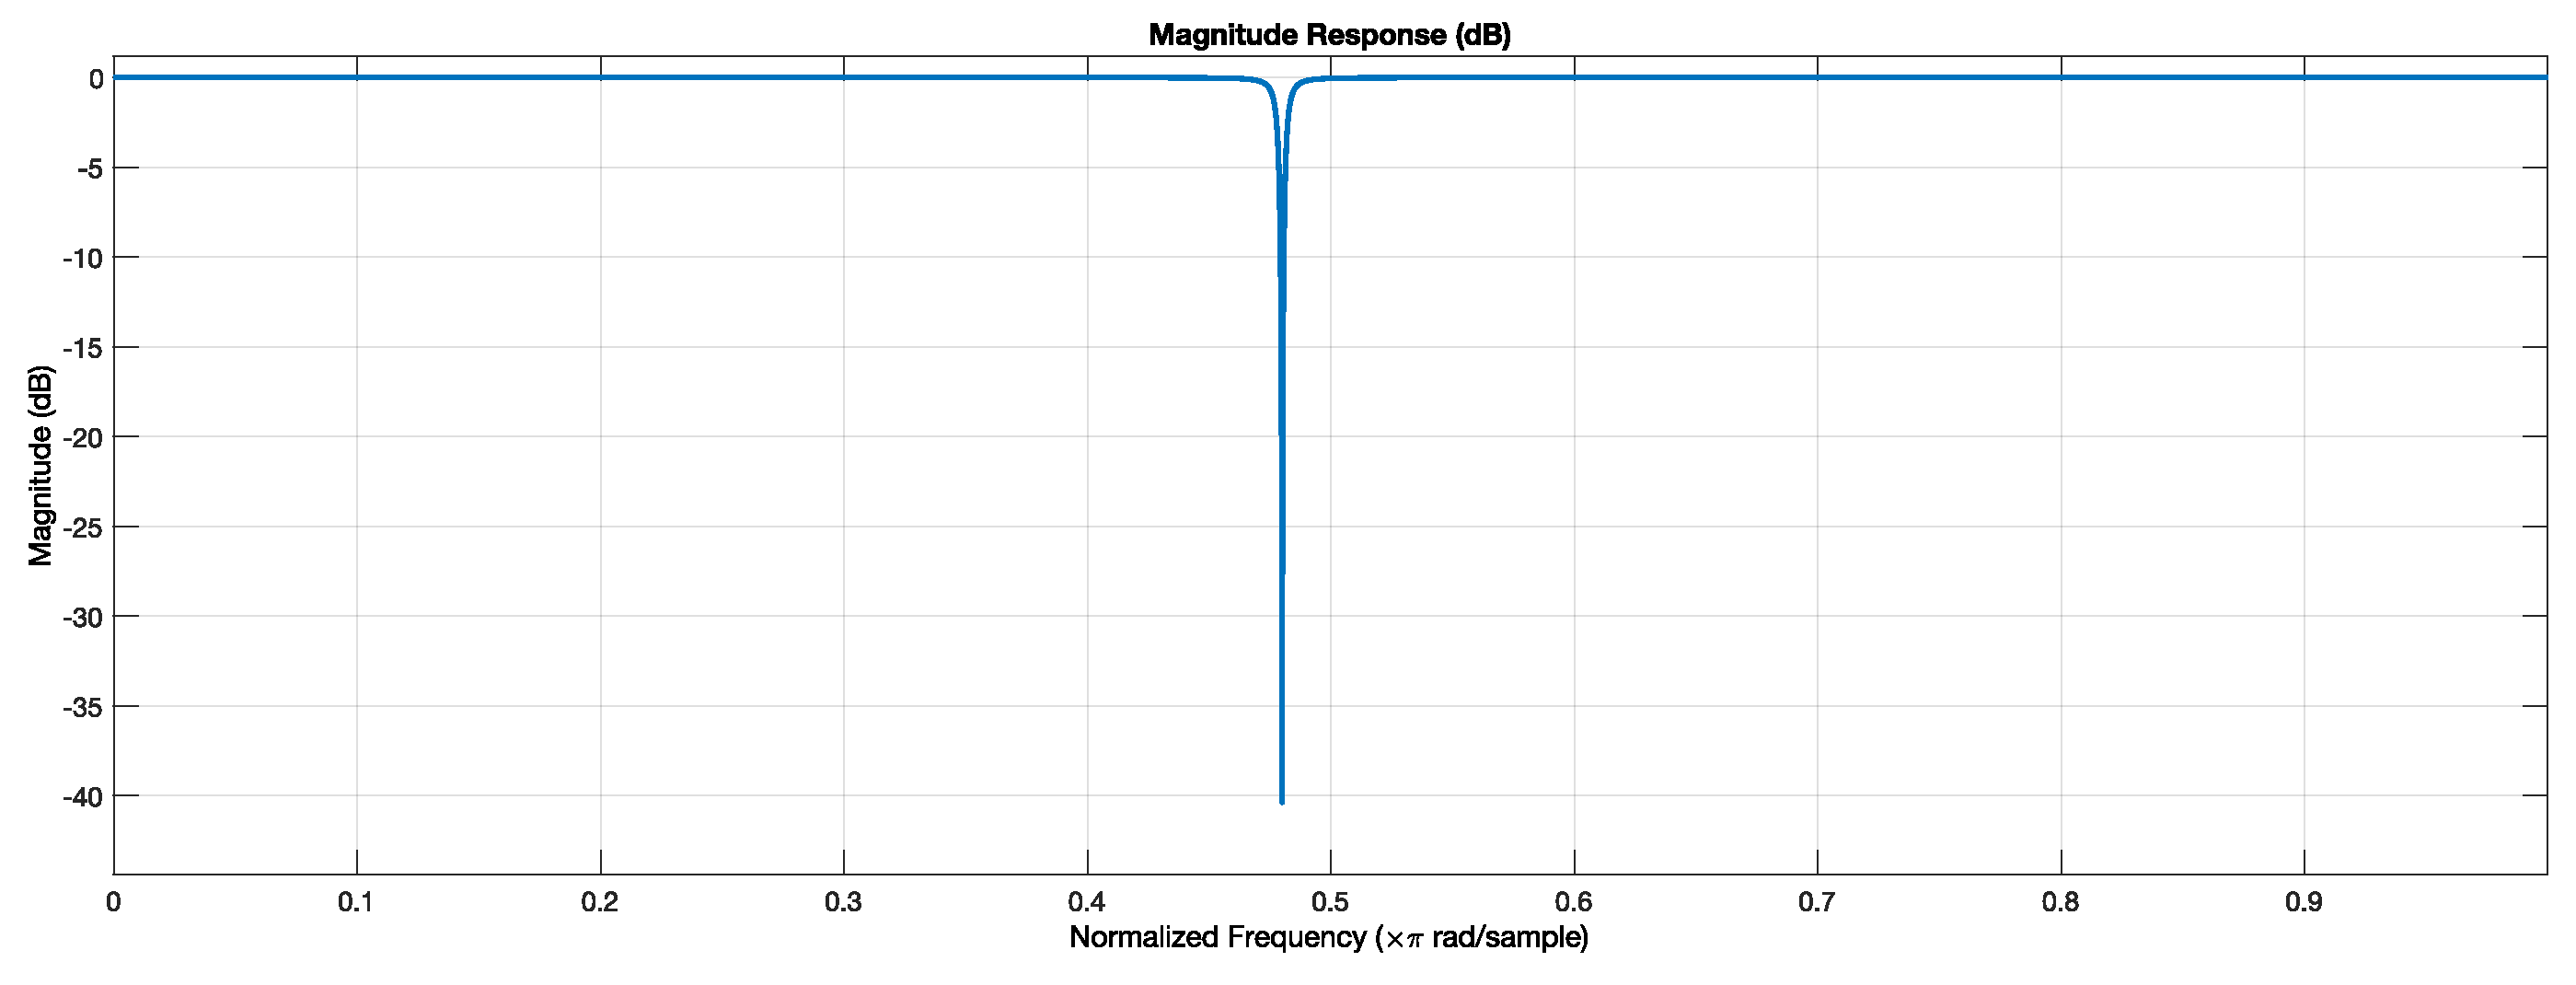
\includegraphics[width=1\textwidth]{resources/pdf/filter_60.pdf}
	    \caption{Magnitude response of the notch filter (\SI{60}{\hertz})}
	    \label{fig:filter_60}
	\end{figure}
	\begin{figure}[H]
	    \centering
	    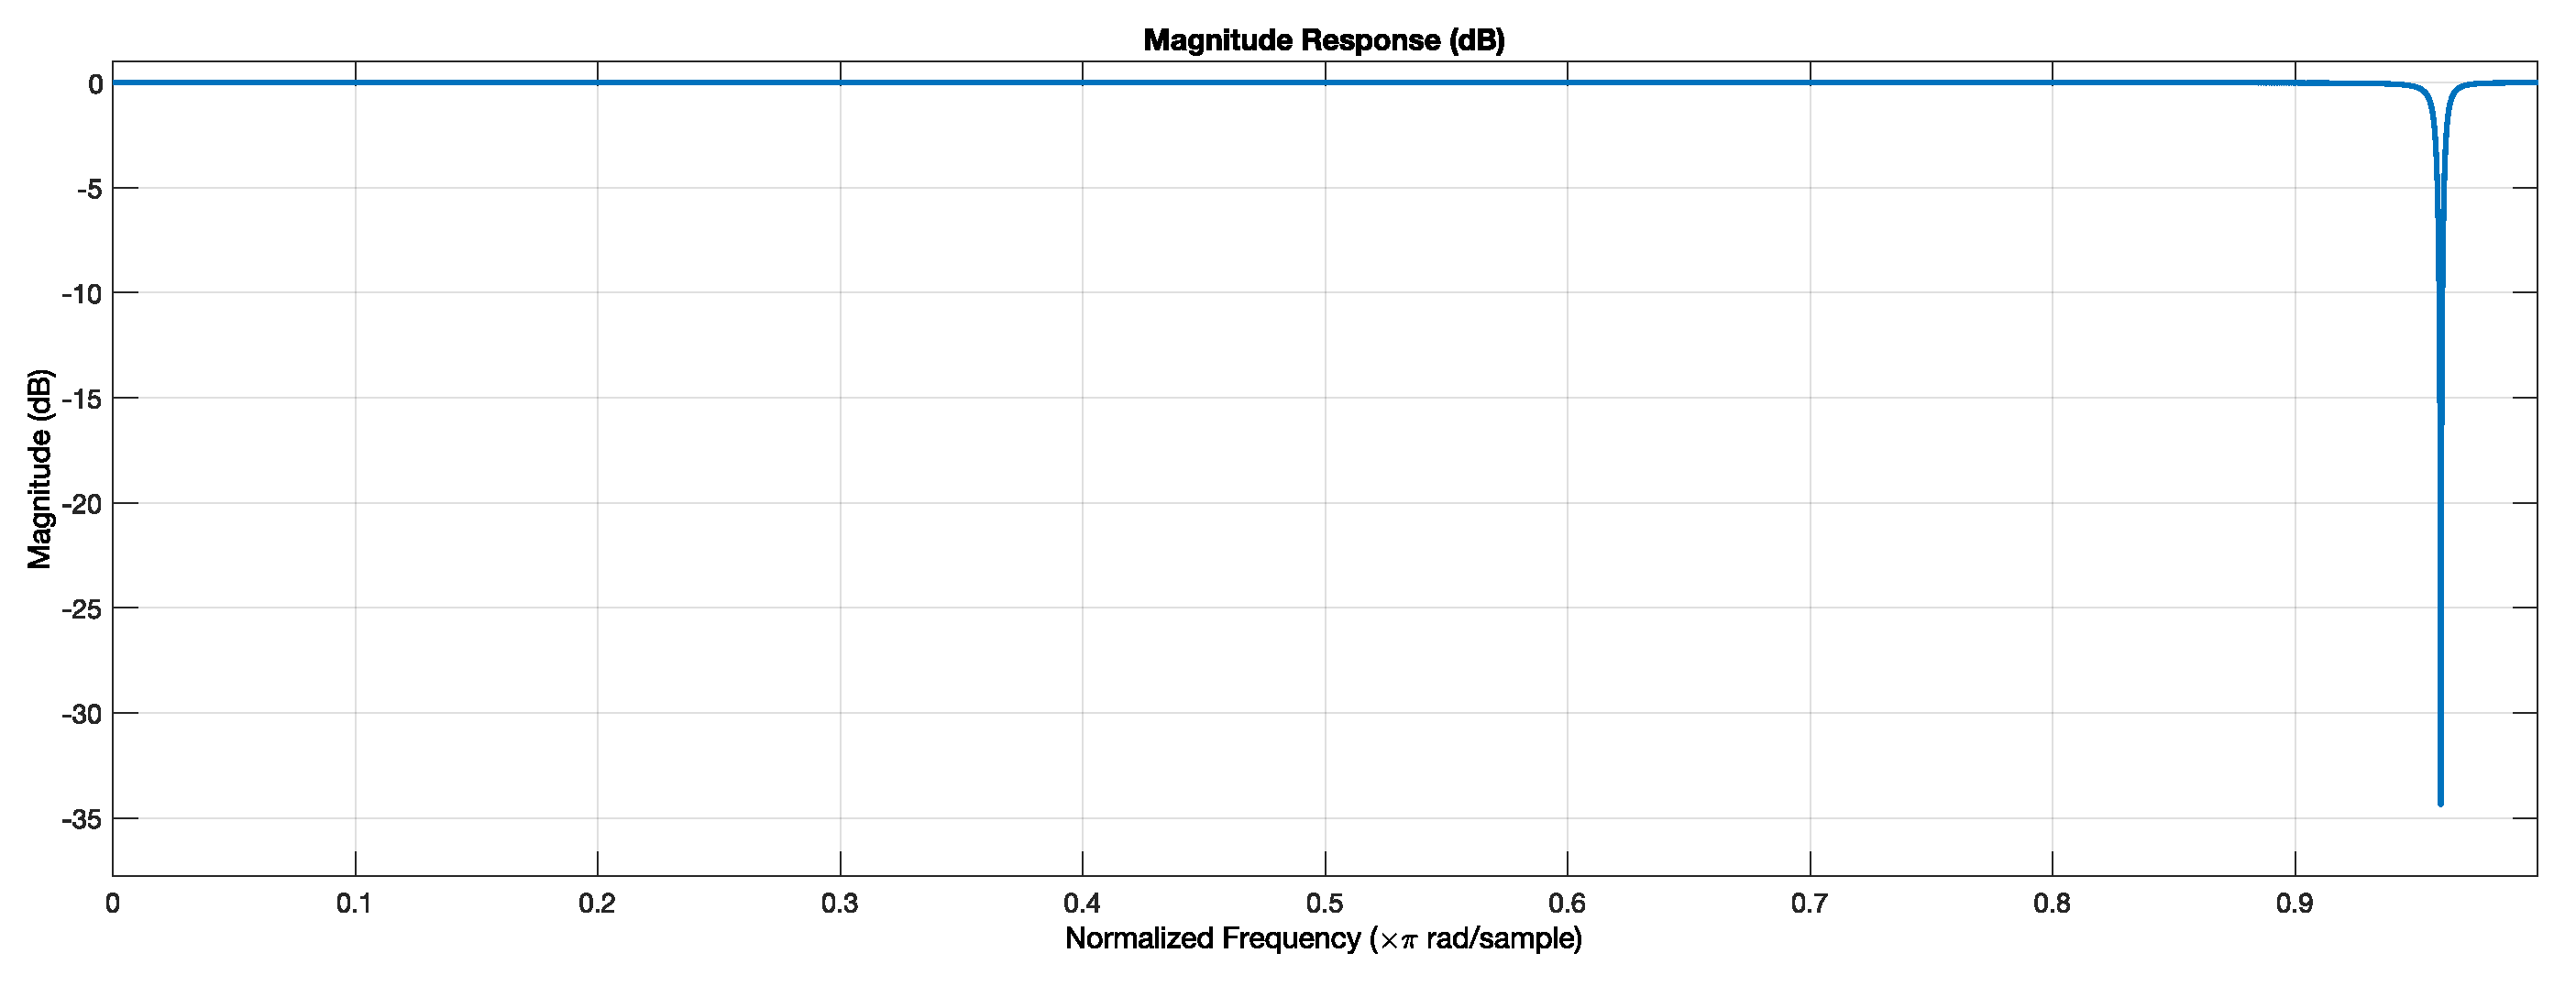
\includegraphics[width=1\textwidth]{resources/pdf/filter_120.pdf}
	    \caption{Magnitude response of the notch filter (\SI{120}{\hertz})}
	    \label{fig:filter_120}
	\end{figure}
	\newpage
	\appendix
	\section{Matlab code}
	\lstinputlisting[style=NFmatlab, caption={Elimination of noise on the signal \texttt{hw2\_electrocardiogram.mat}.}]{resources/m/Q1.m}
\end{document}
